\section{Projekt Terenu}
Projektowanie naszego terenu zaczęliśmy od lokacji startowej, czyli miasta, w którym rozpoczyna się gra. 
Stworzyliśmy spustoszone miasto, które miało oddawać klimat, w jakim został osadzony cały projekt. 
\begin{figure}[H]
	\center
	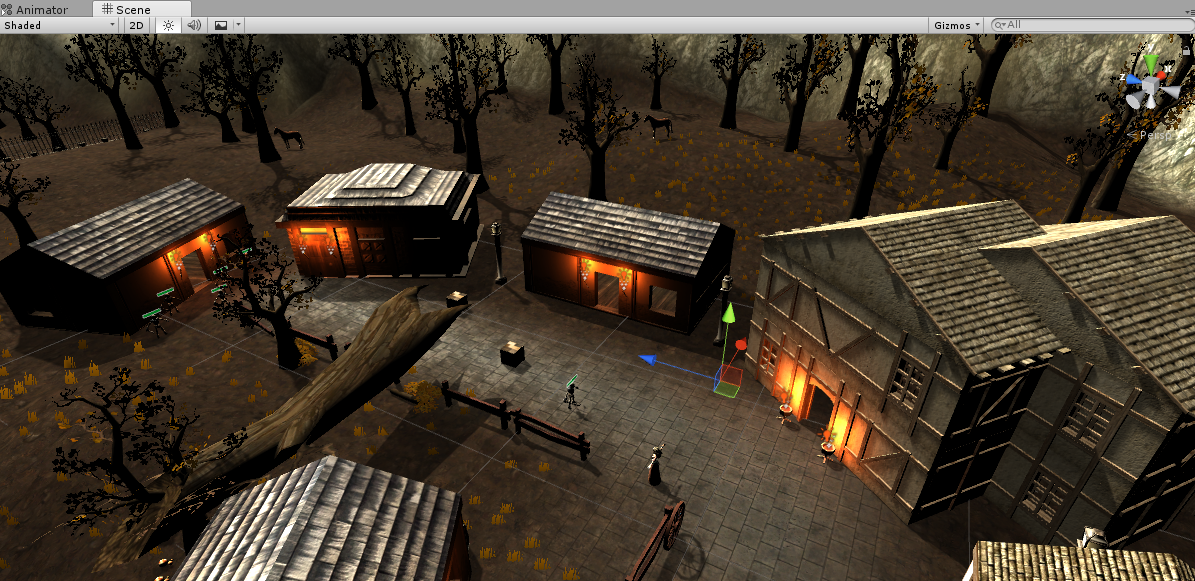
\includegraphics[width=8cm]{scena.png}
	\caption{Początkowa lokacja na scenie, w której bohaterowie rozpoczynają przygodę}
\end{figure}
Na początku rozgrywki napotkamy kilku przeciwników oraz przerażoną kobietę, która wprowadzi nas w świat gry.  
Postaci kierowane przez graczy posiadają określoną rolę, dlatego dalsza część mapy została zaprojektowana z myślą o specjalnych umiejętnościach każdego z nich.
Po drodze możemy spotkać niezliczone grupy przeciwników oraz przeszkody w postaci ukształtowania terenu, które możemy pokonać tylko przy pomocy jednego z bohaterów.
Przez resztę rozgrywki poruszamy się krętą ścieżką, która prowadzi do oazy.
Jest to płaski otwarty teren, na którym bohaterowie będą mogli stoczyć ostateczną walkę ze źródłem swoich problemów.
\begin{figure}[H]
	\center
	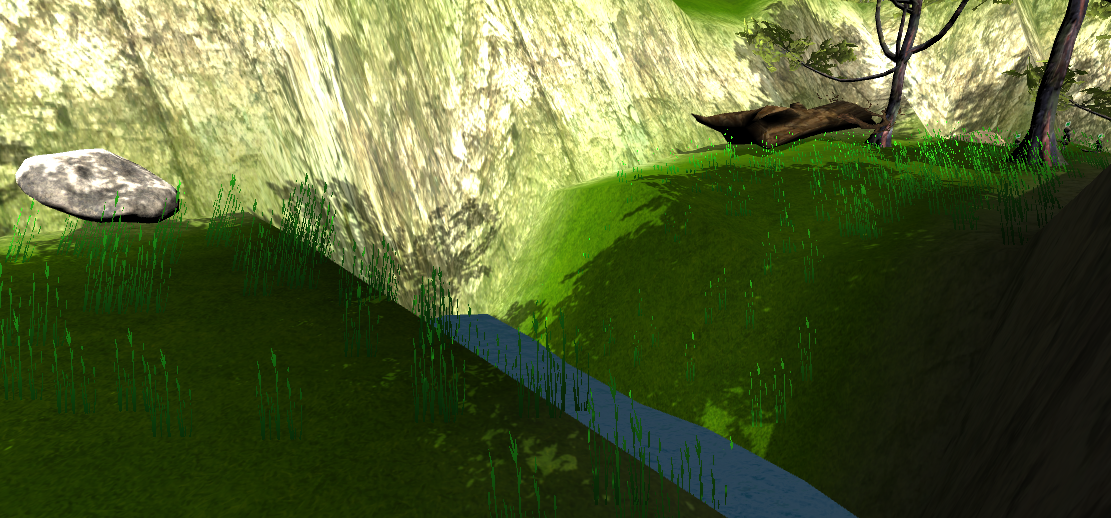
\includegraphics[width=8cm]{scena2.png}
	\caption{Przykładowa przeszkoda w postaci ukształtowania terenu}
\end{figure}